\htwo{Überblick}

\begin{figure}[H]
    \centering
    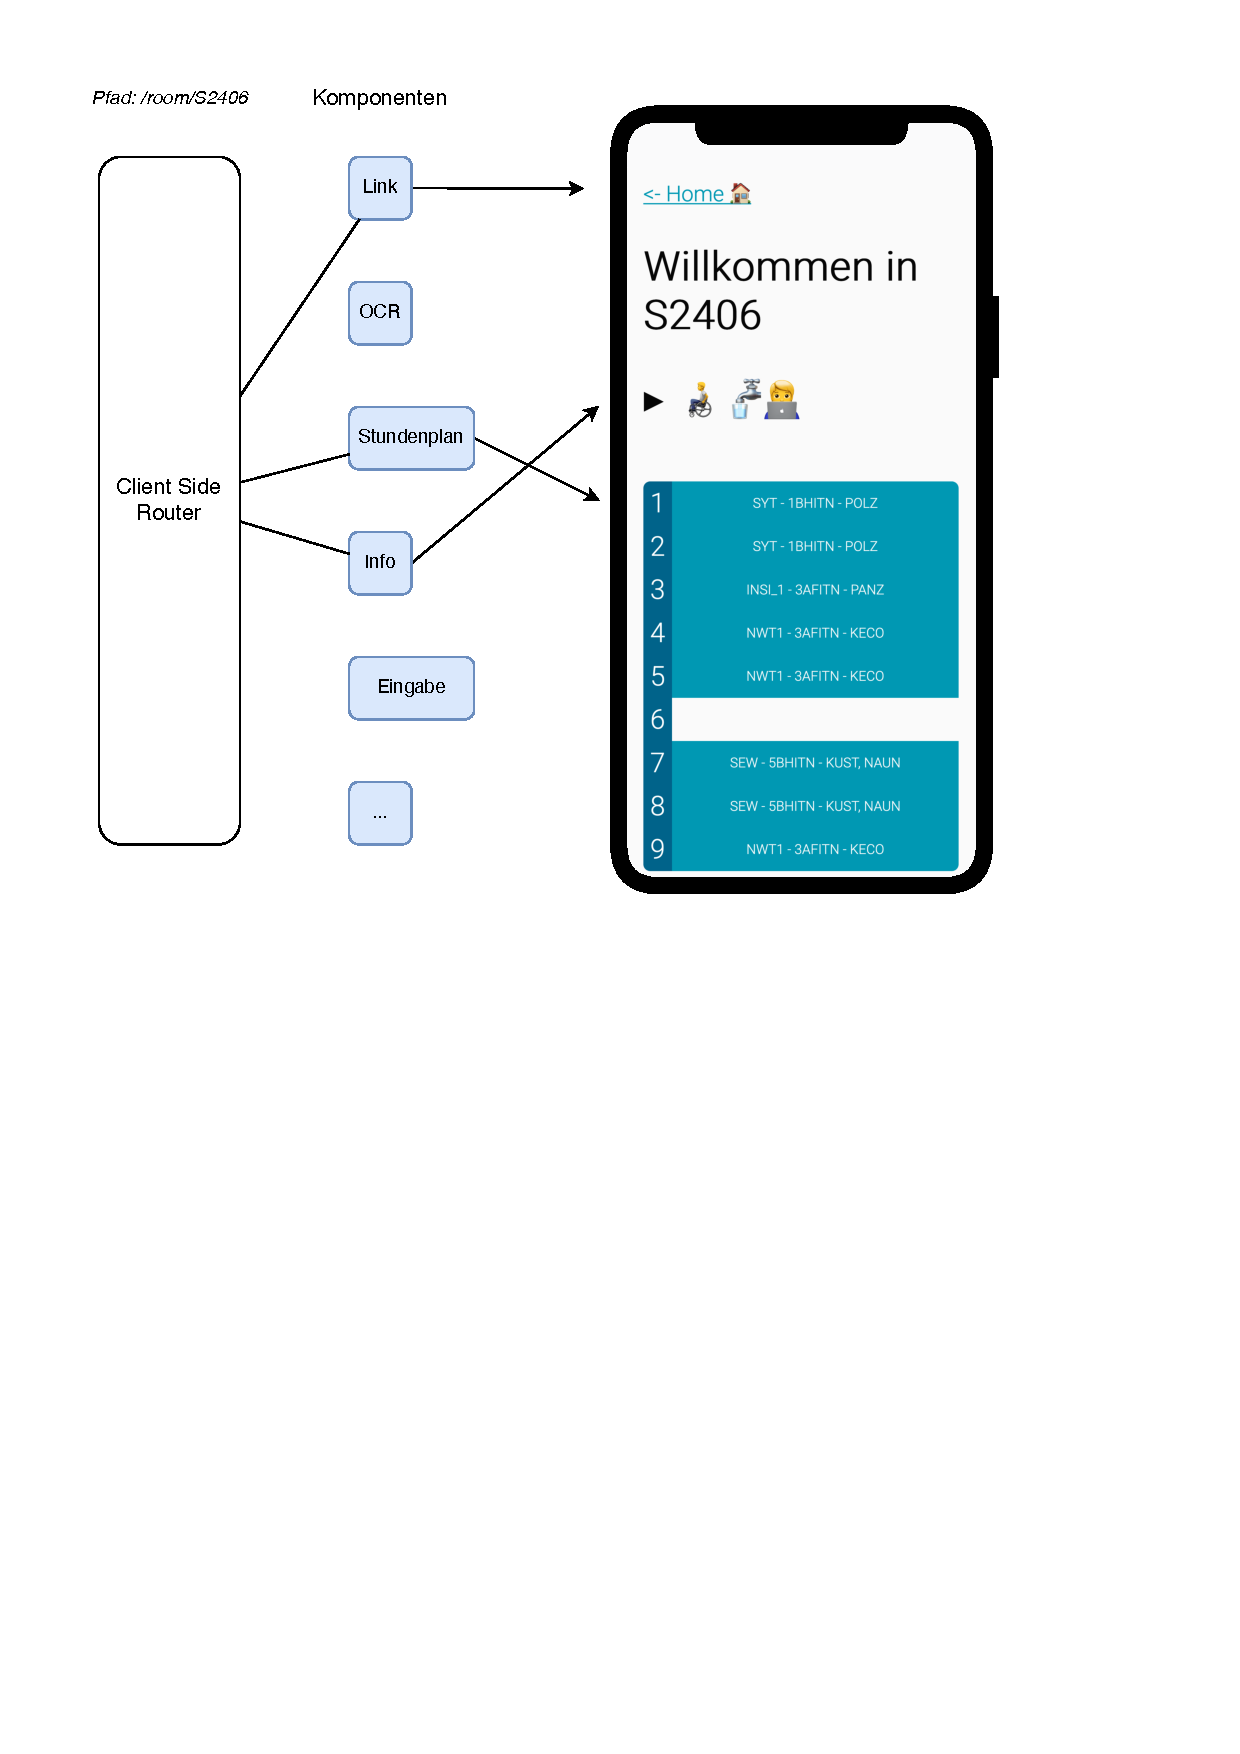
\includegraphics[width=120mm]{media/Intro/client_arch.svg.pdf}
    \caption{Architektur des Clients}
\end{figure}

Der \ZELIA-Client ist eine Web-Anwendung welche in HTML, CSS und Typescript von Grund auf selbst geschrieben ist. Es wird nur eine externe Bibliothek für die Funktionalität der Webseite verwendet, nämlich TesseractJS. Das Tesseract-Projekt ist ein "Open Source"-Softwareprojekt, welches Texte aus Bildern extrahiert. Bei \ZELIA\ wird das benötigt um mit der Smartphonekamera die Raumnummern, zum Beispiel von Türschildern, einzuscannen (siehe Kapitel "Optical Character Recognition" \ref{sec:ocr}, Seite \pageref{sec:ocr}).

Dadurch, dass keine fremde Bibliotheken (außer TesseractJS) verwendet werden, ist die "Frontend-Engine" selbst entworfen und implementiert. Diese "Engine" ist eine Ansammlung an Funktionen, um eine moderne Webseite zu erstellen. Die Anforderungen für diese Bibliothek waren, dass man sie von \ZELIA\ trennen kann und sie somit für jede andere Webseite wiederverwendbar ist. Dafür wurde die Bibliothek komplett unabhängig von dem eigentlichen Projekt geplant. 

Dieses "Frontend Framework" besteht aus zwei logischen Teilen, die nichts miteinander zu tun haben:
\begin{itemize}
    \item Einem Komponentensystem, mit dem man Elemente auf die Webseite hinzufügen und manipulieren kann (siehe Kapitel "WebComponents" -- Implementierung \ref{sec:webcompimp}, Seite \pageref{sec:webcompimp}).
    \item Einem "Frontend Router", welcher dafür zuständig ist Anfragen auf verschiedenen Pfaden zu verarbeiten (siehe Kapitel "Client Side Router" -- Implementierung \ref{sec:csrouterimp}, Seite \pageref{sec:csrouterimp}).
\end{itemize}

In den folgenden Kapiteln werden die Funktionalitäten der Frontend Bibliothek genauer erklärt.